\section{Repository}
Public repository (Given that it is an open source project).
\begin{itemize}
	\item Options comparison (between GoogleCode, GitHub, SourceForge) \\
		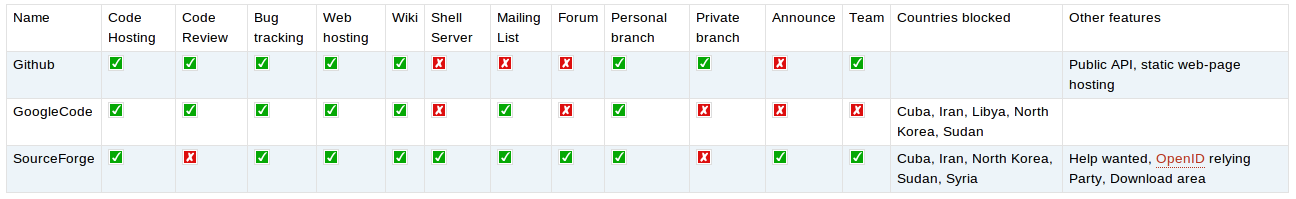
\includegraphics[width=\textwidth]{img/1}
	\item Available version control systems (and other features) \\
		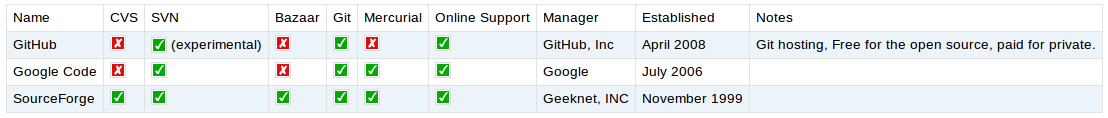
\includegraphics[width=\textwidth]{img/2}
	\item ACS Requirements
		\begin{itemize}
			\item Migration to the new versioning system (keeping changelogs, etc.): There are not suitable tools to convert from CVS to GIT or SVN in 
				a consistent way for large projects such as ACS. We have previously tried to convert ACS to different versioning systems obtaining 
				random loss of patches in the resulting repository. For this reason we need to analyze how this process should be done.
		\end{itemize}
	\item Veredict
		\begin{itemize}
			\item Currently GitHub does not support many version control systems, but they have the most active community (between GitHub, Source Forge 
				and Google Code), and with their Public API potential their growth. So our decision is to choose GitHub. Actually SourceForge has
				more users than Gitb Hub, but we decided according with this ratio $\frac{number\_of\_users}{years\_operatting}$.
		\end{itemize}
	\item Policies
		\begin{itemize}
			\item Branching: Reason to branch: experimental development, release maintenance.
			\item Tagging: Reason to tag: release tag.
			\item Merge: UTFSM direct, Stable Community pull request, other contributors: patch mail.
			\item Permissions
				\begin{itemize}
					\item Admin: UTFSM group.
					\item Write: UTFSM group, Stable community (pull request review).
					\item Read: anyone.	
				\end{itemize}
			\end{itemize}
\end{itemize}
